%!TEX root = ../thesis.tex

\chapter{Background}
\label{ch:background}

This thesis integrates open problems in population genetics and evolutionary biology with powerful tools from applied topology.
As few readers will likely have substantial exposure to both fields, we devote this initial chapter to prelimaries and motivation.
Exposition required for specific results will be found in the individual chapters.

\section{Biology}

In this section we present biological background.
This section is intended to motivate the problems discussed.
More specific background relevant to the applications described in Part \ref{part:application_microorganism} and Part \ref{part:applications_human} is presented in those Parts.

What do we mean by horizontal and vertical evolution?
Vertical, or clonal, evolution is mediated by stochastic mutations over multiple generations.
Vertical evolution is consistent with a phylogenetic tree.

\subsection{Population Genetics}

Mathematical population genetics is concerned with properties of populations as they are subject to evolutionary forces over long time scales.
These forces include natural selection, genetic drift, mutation, and recombination.
Historically the input data for population genetics models was comparative studies of allele frequencies across populations.
Large-scale genome surveys 
Develop genealogy.
Look at population structure.

\subsection{Phylogenetics}

Phylogenetics is concerned with relationships among species as inferred from evolutionary characters.

Phylogenetics is how you build a tree from evolutionary characters.

Start with sequences.
Perform an alignment.
From an alignment, one can then directly use parsimony or likelihood approaches.
Alternatively, one can compute a matrix of pairwise distances and then construct a tree that best approximates these distances.
Most relevant to this thesis are the distance-based approaches (because they can be viewed as finite metric spaces amenable to topological analysis).
Only in the case of perfectly additive data will a tree be able to exactly fit the matrix.
Identifying the pairwise distance matrix with a its finite metric space representation allows most of the results described here.

Include discussion of rooted vs unrooted.

\subsection{Distance Matrix Methods}

Introduced by Cavalli-Sforza and Edwards in 1967 \cite{CavalliSforza:1967th} and Fitch and Margoliash in 1967 \cite{Fitch:1967we}.
Compute a matrix of pairwise distances and then find the tree that best approximates those distances.
Weighted and unweighted least squares.
UPGMA.
Neighbor joining is now the most common distance-matrix approach because it can perfectly reconstruct an additive tree.
Neighbor joining was introduced by Saitou and Nei in 1987 \cite{Saitou:1987wo}.

There are limitations of distance based methods.
Do not use all the information.

Need to include discussion of metrics on aligned sequences.

\subsection{The Coalescent}

The coalescent process is a stochastic model that generates the genealogy of individuals sampled from an evolving population \cite{Wakeley:2009}.
The genealogy is then used to simulate the genetic sequences of the sample.
This model is essential to many methods commonly used in population genetics.
Starting with a present-day sample of $n$ individuals, each individual's lineage is traced backward in time, towards a mutual common ancestor.
Two separate lineages collapse via a coalescence event, representing the sharing of an ancestor by the two lineages.
The stochastic process ends when all lineages of all sampled individuals collapse into a single common ancestor.
In this process, if the total (diploid) population size $N$ is sufficiently large, then the expected time before a coalescence event, in units of $2N$ generations, is approximately exponentially distributed:
\begin{equation}
P(T_{k}=t) \approx \binom{k}{2} e ^{-\binom{k}{2} t},
\end{equation}
where $T_k$ is the time that it takes for $k$ individual lineages to collapse into $k-1$ lineages.

After generating a genealogy, the genetic sequences of the sample can be simulated by placing mutations on the individual branches of the lineage.
The number of mutations on each branch is Poisson-distributed with mean $\theta t / 2$, where $t$ is the branch length and $\theta$ is the population-scaled mutation rate.
In this model, the average \emph{genetic distance} between any two sampled individuals, defined by the number of mutations separating them, is $\theta$.

The coalescent with recombination is an extension of this model that allows different genetic loci to have different genealogies.
Looking backward in time, recombination is modeled as a splitting event, occurring at a rate determined by population-scaled recombination rate $\rho$, such that an individual has a different ancestor at different loci.
Evolutionary histories are no longer represented by a tree, but rather by an \emph{ancestral recombination graph}.
Recombination is the component of the model generating nontrivial topology by introducing deviations from a contractibile tree structure, and is the component which we would like to quantify.
Coalescent simulations were performed using \texttt{ms} \cite{Hudson:2002}.

% \begin{figure}
% \begin{center}
% \centerline{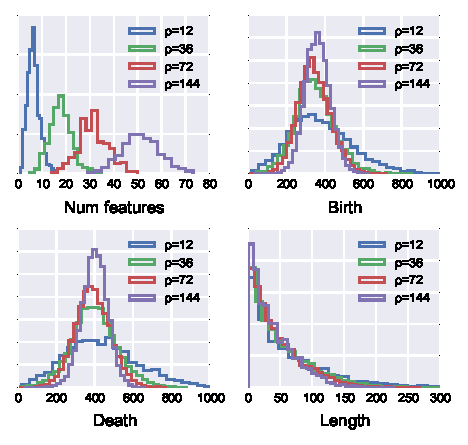
\includegraphics[width=\columnwidth]{./fig/coalescent_sims.pdf}}
% \caption{Distributions of statistics defined on the $H_1$ persistence diagram for different model parameters. Top left: Number of features. Top right: Birth time distribution. Bottom left: Death time distribution. Bottom right: Feature length distribution. Data generated from $1000$ coalescent simulations with $n=100$, $\theta=500$, and variable $\rho$.}
% \label{fig:coalescent_sims}
% \end{center}
% \end{figure}

\subsection{Horizontal Gene Transfer}

Here we should include discussion of nonvertical evolutionary processes.
This will include references to Doolittle, Koonin, Gogarten.
Lateral Gene Transfer.
Species Trees and Gene Trees.
Recombination and reassortment.
We will want to include discussion of 

%%%%%%%%%%%%%%%%%%%%%%%%%%%%%
% TOPOLOGICAL DATA ANALYSIS %
%%%%%%%%%%%%%%%%%%%%%%%%%%%%%

\section{Mathematics}

Topology is the study of shape.
Algebraic topology associates algebraic structures to notions of shape.
Computational topology provides tools of computing invariants.
Topological data analysis is the name for the field that has emerged from this work, offering a suite of approaches for analyzing real world data using topological information.

Algebriac topology associates algebraic structures to qualitative notions of shape.
Principle tool is group theory.
Groups count connected components.

\subsection{Topology}

Topology: characterize properties of spaces invariant under continuous deformation.

\subsection{Algebraic Topology}

In this section we give background sufficient to define homology for our purposes, before moving on to applied topology and persistent homology.
A more thorough exposition of algebraic topology can be found in [HATCHER].

\subsubsection{Simplicial Complex}

Associate a collection of algebraic objects with a topological space.
Quantify global properties of space.
Homotopy and Homology.
Homology: properties of chains composed of oriented simplices
Elements of homology groups are cycles (chains with vanishing boundary).
Two k-cycles are homologous if they differ by the boundary of a (k+1)-chain.
Glue together simplices : simplicial complex.

\begin{enumerate}
\item Any face of a simplex in K is also in K
\item The intersection of any two simplices in K is a face of both 
\end{enumerate}

Incidence matrix representation...

\subsubsection{Chains, cycles and boundaries [rephrase]}

Boundary operator $\partial_{k}:C_{k}\rightarrow C_{k-1}$.
Action of boundary operator on a simplex $\sigma$ is defined as: 

\begin{equation}
\partial_{k}\sigma = \displaystyle\sum_{i}(-1)^{i}[v_{0},v_{1},...,\hat{v}_{i},...,v_{n}].
\end{equation}

A chain $C\in C_{k}$ is called a cycle if $\partial_{k}C=0$.
Chain with empty boundary.
Set of cycles forms a group

Boundary operator defines a chain complex $C_{*}$:

\begin{equation}
\dots \overset{\partial_{n+1}}{\longrightarrow} C_n \overset{\partial_{n}}{\longrightarrow} C_{n-1} \overset{\partial_{n-1}}{\longrightarrow}  ... \overset{\partial_{2}}{\longrightarrow} C_n \overset{\partial_{1}}{\longrightarrow} C_{n-1} \overset{\partial_{0}}{\longrightarrow}  0
\end{equation}

Important property:

\begin{equation}
\partial_{k-1}\partial_{k} = 0 \forall k
\end{equation}

Intuitively, a boundary has no boundary.

$C$ is the set of 
The $k$-th cycle group is $Z_{k}=\ker \partial_{k}$.
$Z_{k}$ defines the set of all cycles of dimension $k$.
$B_{k}$ defines the set of all boundaries of dimension $k$.
That is, elements of $B_{k}$ serve as boundaries of $(k+1)$-chains.


TDA+PH: number and type of holes. which holes are essential and which are unimportant.

Basically get to the point where can define homology.
Chain complex.
Boundary operators
Work only over $\mod 2$ Homology (0,1) coefficients.
Torsion observed in teh image patch data set, but no reason to think it is present biologial data sets we examine.

\subsubsection{Homology Groups}

Simplical homology.
Abelian groups.
First homology group: abelianization of the fundamental gorup.
Quotient group

Recalling out definition of the boundary and cycle groups, define a quotient group

\begin{equation}
H_{k} = Z_{k} / B_{k} = \ker\partial_{k} / \im\partial_{k+1}
\end{equation}

Closed chains (cycles) up to boundary of higher dimensional cycles.
Elements are classes of homologous cycles.

\begin{figure}
\centering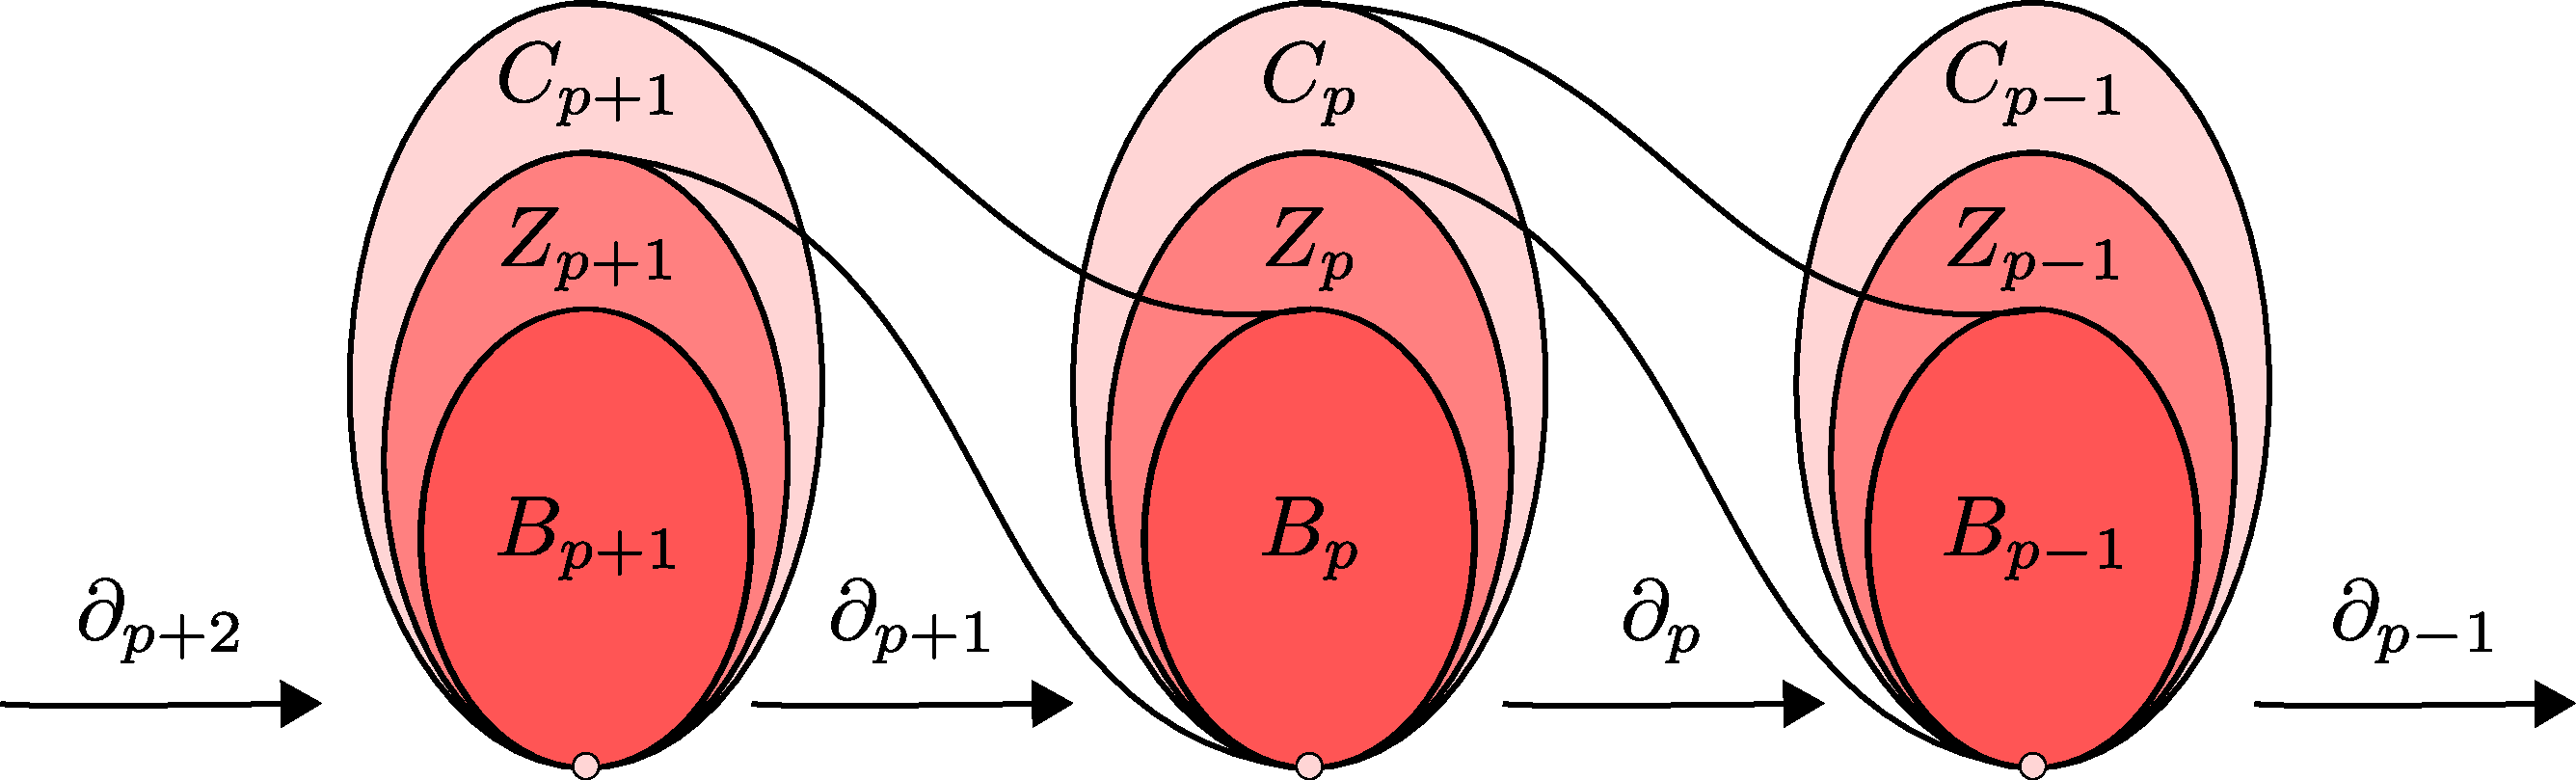
\includegraphics[width=\columnwidth]{./fig/FASY_chain_complexes.pdf}
\caption{Relationship between chain and cycle and homology. Adapted (``Adapted'') from Fasy.}
\label{fig:chain_complexes}
\end{figure}

\subsection{Simplicial Complexes}

Simplex: generalization of triangle or tetrahedron to arbitraty dimensions. [see Zomorodian].
k-simplex: k-dimensional polytope which is the convex hull of k+1 vertices.
Faces. Boundary.
Simplicial complex: collection of simplcies.
Set of vertices: simplex.
Vertices. Dimension.
Abstract Simplicial Complex.

The \Cech complex consists of the set of simplices $\sigma$ with vertices $v_{1},...,v_{k}\in S$ such that

\begin{equation}
\displaystyle\cap_{i}^{} B(v_{i},\epsilon)\neq0
\end{equation}

Cech Complex.
Rips Complex.

\section{Topological Data Analysis}

Topological Data Analysis (TDA) studies structure in high-dimensional data such as connectedness and the presence of holes.
In practice, we observe only a sample of data points, from which we wish to infer an underlying model or generating principle.
TDA first builds topological complexes from data, then measures informative properties of these complexes. 
Persistent homology (PH) is a method from TDA that uses algebraic topology to compute quantitative properties in data, including connectedness and the presence of holes (see Box 1).

Make a connection with graph theory (see Horak). Prgoram: encode data as simplicial complex, combinatorial version of a topological space, properties studied from combinatorial, topological, algebraic perspective.

For excellent review of topological data analysis, see the reviews.
Start with point cloud data.
Built a filtration.
Filtration is a nested set of simplical complexes.

\subsection{Finite Metric Spaces}

Finite metric spaces are really interesting objects of study.
Lots of good work on embedding finite metric spaces, see Matousek.
Metric space with a finite number of points.
Combinatorics, geometric, and algorithms.
In topological data analysis, our spaces of interest are finite metric spaces.

\subsection{Mapper}

Condensed Representations.
Exploratory data analysis.

Can compare to dimensionality reduction.
But is basically clustering.
Reeb graph


\subsection{Persistent Homology}
\label{subsec:persistent_homology}

How to extend homology to finite metric spaces?
Data -> Sets of complexes -> Vector spaces

We summarize persistent homology from the perspective of an end-user.
For detailed background, see the reviews \cite{Carlsson:2009a,Ghrist:2008} and the books \cite{Edelsbrunner:2010,Zomorodian:2005b}.
In brief, persistent homology computes topological invariants representing information about the connectivity and holes in a dataset.
A dataset, $S=(s_{1},\ldots,s_{N})$, is represented as a point cloud in a high-dimensional space (not necessarily Euclidean).
From the point cloud, a nested family of simplicial complexes, or a filtration, is constructed, parameterized by a filtration value $\epsilon$, which controls the simplices present in the complex.
The two most common ways of constructing a simplicial complex at each $\epsilon$ are the \Cech complex and the Vietoris-Rips complex.
The filtration is represented as a list of simplices defined on the vertices of $S$, annotated with the $\epsilon$ at which the simplex appears.
Given a filtration, the persistence algorithm is used to compute homology groups.
The $0$-dimensional homology ($H_0$) represents a hierarchical clustering of the data.
Higher dimensional homology groups represent loops, holes, and higher dimensional voids in the data.
Each feature is annotated with an interval, representing the $\epsilon$ at which the feature appears and the $\epsilon$ at which the feature contracts in the filtration.
These filtration values are the \emph{birth} and \emph{death} times, respectively.

The topological invariants in the filtration can be concisely represented in a barcode diagram, a set of line segments ordered by filtration value on the horizontal axis.
In the barcode diagram,

The topological invariants in the filtration can be concisely represented in a barcode diagram, a set of line segments ordered by filtration value on the horizontal axis (Figure XXX).

Invariants can be equivalently represented by a persistence diagram, a scatter plot with the birth time on the horizontal axis and the death time on the vertical axis.

Connected components.
Loops.
Voids.

TOPOLOGICAL DATA ANALYSIS BABY!

The intuition behind persistent homology is that is that good or interesting features will persist over longer scales
That is, they will be more robust.
In the barcode diagram this corresonds to long bars, and in the persistence diagram, this corresponds to points far from the diagonal.
Invariants that persist for only short scales are likely to be noise or artifacts of incomplete sampling.
The questions of how to rigorously determine what makes a good interval is an open question that is currently being addressed by a number of different groups.
We discuss this further in Section \ref{subsubsec:ph_statistics}.

\subsubsection{The Persistence Algorithm}

While we act mostly as an end-user of persistent homology in this thesis, the algorithmics behind efficient computations of homology are interesting and worth including for comprehensiveness.
Computing persistent homology is an exercise in linear algebra.
The initial algorithms first induce a matching on a set of simplices.
This was Zomorodian and is the implementation used in Javaplex and Dionysus.
Then you reduce a couple of matrices.
You can read off each bar and its represetnative cycle from looking at the zeros on this one particular matrix.
It's pretty nifty.

More advanced algorithms have been developed that compute simplicial collapses: recognizing that the size of the simplciial set is often the limiting factor here, they collapse simplicies into simpler structures that will have identical homology.
This uses Discrete Morse Theory and is the idea behind implementations such as Perseus.

Include only simple implementation for $Z2$

Several packages for computing persistent homology have been developed [Dionysus, Javaplex, Guidi, phom] and TDA frontend for R.
Persistent homology is computed using Dionysus \cite{Morozov:2012}.

\subsubsection{Stability}
\label{subsubsec:ph_stability}

What happens if we perturb the original data slightly?
Will bars change?
Will new bars be formed?
Stability result determined how a change in $D\rightarrow D'$ takes us to $H\rightarrow H'$.

Couple of comments about different distances on topological space: Hausdorff, Gromov-Hausdorff.
Distances between barcodes: Bottleneck, Wasserstein. Matchings.

conclusion: small perturbations in data can only produce small changes in the barcode.

\subsubsection{Statistical Persistent Homology}
\label{subsubsec:ph_statistics}

Currently the cutting edge in TDA.
Primarily motivated
Cutting edge in TDA.
Primarily motivated by the idea that there is a true topology and we are given a finite sample of it.
We are motivated by a slightly different problem in this thesis.
We briefly discuss these results.
Persistence Landscapes.
Bootstrap resampling.

\subsubsection{Multidimensional Persistence}
\label{subsubsec:ph_multidim}

Filtrations along different dimensions.
Prototypical example: density and distance.
Include a bit of discussion of Lesnick's ideas.

Our case is going to be slightly different.
We will consider a set of points annotated with different metrics that we can put on it which will induce different homologies.
Then we will see what happens we interpolate between those different metrics.

\section{Space of Phylogenetic Trees}

(This section may or may not be moved, but I want to get it on the page.)
Studies of tree space were initiated by Billera, Holmes, and Vogtmann in \cite{Billera:2001tv}.
Each point represents an unrooted binary tree with L leaves and positive branch lengths.
Number of interior edges $r=L-3$, a particular daditive tree can be plotted as a point in the positive open orthant $(0,\infty)^{r}$.
A single orthan corresponds to a single tree topology.


four point condition.

\subsection{Number of Trees}

[should be in phylogenetics section].
Unrooted, bifurcating, labeled trees
Multiple tree topologies can exist.
Number of unrooted bifurcating trees with $L$ leaves is $(2L-5)!!$.

Number of tree topologies explodes with number of leaves.
Fitch quote: more than 20 species, more than Avogadro's number of topologies.
Phylogeny can be seen as projecting onto the space of trees.